\documentclass[english,a4paper,12pt]{report}
\usepackage{mypackage}

\title{Electrodynamics}

\author{Haydn Cheng}

\date{\today}

\begin{document}
\maketitle
\tableofcontents
    
\chapter{Basic Concepts and Sign Conventions}

\section{Ohm's Law}

To make a current flow, you have to push on the charges. How fast they move, in response to a given push, depends on the material's conductivity \(\sigma \) defined by 

\begin{equation}
    \vb{J} = \sigma \vb{f} , \label{ohm} 
\end{equation}

where \(\vb{J} \) is the volume current density defined by \(\displaystyle \vb{J} = \frac{\vb{I} }{A} \) and \(\vb{f} \) is the force per unit charge. The reciprocal of \(\sigma \), \(\displaystyle \rho =\frac{1}{\sigma } \), on the other hand, is called the resistivity.  

For our purposes, it is usually an electromagnetic force that does the job. In this case, the above equation becomes

\begin{equation}
    \vb{J} = \sigma (\vb{E} + \vb{v} \cross \vb{B} ).
\end{equation}

Ordinarily, the velocity of the charges is sufficiently small that the second term can be ignored, so we get

\begin{equation}
    \vb{J} = \sigma \vb{E} ,
\end{equation}

which is the famous Ohm's law, though it is only a special case of \(\vb{J} = \sigma \vb{f} \), which is actually just the definition of conductivity. In fact it is not really a true law, in the sense of Coulomb's or Ampere's, rather it is a ``rule of thumb'' that applies pretty well to many substances.

Note that the force \(\vb{f}\) does not include the ``resistive force'' in the resistor because it is not really a force but the constant instant collisions between the charges and the material can be modelled as a force, which cancels out with the external force \(\vb{f}\), to give a constant current.

It is a little like this: suppose you are driving down a street with a stop sign at every intersection, so that, although you accelerate constantly in between, you are obliged to start all over again with each new block. Your average speed is then a constant, in spite of the fact that (except for the periodic abrupt stops) you are always accelerating. If the length of a block is \(\lambda \)  and your acceleration is \(a\), the time it takes to go a block is \(\displaystyle t=\sqrt{\frac{2\lambda }{a} }\) and hence your average velocity is \(\displaystyle \avg{v} = \frac{1}{2} at = \sqrt{\frac{\lambda a}{2} }  \). 

But this is not good either, since it says that the velocity is proportional to the square root of the acceleration and therefore that the current should be proportional to the square root of the field. The twist is that the charge in practice are already moving very fast because of their thermal energy but they have random directions and average to zero. The drift velocity, which is what we are concerned about since it is what related to the current is the extra tiny bit, so the time between collisions is actually much shorter than what we suppose. In this case, the current density is

\begin{equation}
    \vb{J} = nfq\avg{v} = nfq \left( \frac{1}{2}at \right) = nfq \left( \frac{1}{2}a\frac{\lambda}{v_{\text{thermal} } }  \right) = \left( \frac{nf\lambda q^2}{2mv_{\text{thermal} } }  \right) \vb{E}  
\end{equation}

where \(n\) is the number of molecules per unit volume and \(f\) is the number of free electrons per molecule. So \(\vb{J} \) is indeed proportional to \(\vb{E} \).  

In practice, we usually assume wires are perfect conductor with \(\sigma \rightarrow \infty\), so \(\displaystyle \vb{E} = \frac{\vb{J} }{\sigma } =0\) in wires and thus can be treated as equipotentials. Resistors, by contrast, are made from poorly conducting materials. 
\todo{example7.2 have both resistance and capacitance (in parallel), maintain at V = connect to battery, example 7.3} 

For steady currents and unifrom conductivity, Ohm's law implies that 

\begin{equation}
    \curl{\vb{E} } = \frac{1}{\sigma } \curl{\vb{J} } = 0  
\end{equation}
 
and therfore the charge density is zero and any unbalanced charge resides on the surface.



\section{Electromotive Force}

\subsection{The General Definition}

A circuit in the most general sense is simply a closed loop \(C\). The definition of the elctromotive force of this circuit is the line integral \(\vb{f} \) along \(C\) (taken in the positive sense of \(C\), which is usually anticlockwise)  

\begin{equation}
    \mathcal{E} = \oint_{C}  \vb{f} \cdot d \vb{l} .
\end{equation}

\begin{center}
    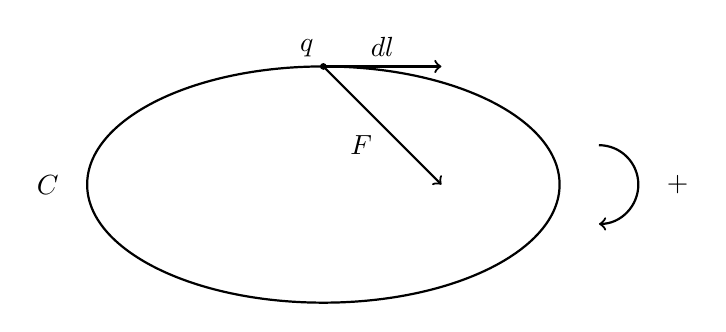
\begin{tikzpicture}
        % Draw the elliptical loop C
        \draw[thick] (0,0) ellipse (3cm and 1.5cm);
        
        % Label the loop C
        \node at (-3.5,0) {$C$};
        
        % Place the charge q and draw the vectors
        \filldraw (0,1.5) circle (1pt) node[above left] {$q$};
        
        % Draw dl vector
        \draw[->, thick] (0,1.5) -- (1.5,1.5) node[midway, above] {\(d \vb{l} \) };
        
        % Draw F vector
        \draw[->, thick] (0,1.5) -- (1.5,0) node[midway, below left] {\(\vb{F} \) };
        
        % Draw the circular arrow with a plus sign
        \draw[->, thick] (3.5,0.5) arc[start angle=90, end angle=-90, radius=0.5cm];
        \node at (4.5,0) {\(\boldsymbol{+} \) };
    \end{tikzpicture}
\end{center}

This formula is basically identical to the definition of work done, where \(W = \int_{a}^{b} \vb{F} \cdot d \vb{s}  \), just that we always perform loop integral for \(\mathcal{E}\) and the forces we use for calculating emf is per unit charge. Therefore, emf can also be interpreted as the work done by the net force per unit charge around a circuit.\footnote{This intepretation is flawed when the circuit itself is also in motion, since the infinitisimal displacement of charges would then not be equal to the infintisimal length element of the circuit, so \(d \vb{l} \) in emf is not equals to \(d \vb{s} \) in work done. We will deal with this problem when discussing generators.}

There are really two force involved in driving charges around a circuit: the source force, \(q \vb{f} _{s}  \), which is usually confined to one portion of the loop (a battery, say) and an electromagnetic force, \(q(\vb{E} + \vb{v} \cross \vb{B} ) \).

\begin{equation}
    \vb{f} = \vb{f} _{s} + \vb{E} . 
\end{equation}

The physical agency responsible for \(\vb{f} _{s} \)  can be many different things: in a battery it is a chemical force; in a piezoelectric crystal, mechanical pressure is converted into an electrical impulse; in a thermocouple it is a temperature gradient that does the job; in a photoelectric cell it is light; and in a Van de Graaff generator the electrons are literally loaded onto a conveyer belt and swept along. 

\subsection{Motional Emf}
Consider a loop of wire moving inside a static magnetic field \(\vb{B} (\vb{r} )\). Let \(\vb{v} \) be the velocity of the element \(d \vb{l} \) relative to our inertial frame of reference (lab frame). Let \(\vb{v} '\) be the velocity of \(q\) relative to \(C\), which must be directed along \(d \vb{l} \) since \(q\) cannot escape the wire in \(C\)'s frame. Thus the total velocity of \(q\) relative to us is \(\vb{v} _{\text{tot} } = \vb{v} + \vb{v} ' \). The force from the magnetic field on \(q\) is then

\begin{equation}
    \vb{F} = q(\vb{v} _{\text{tot} } \cross \vb{B} ) = q (\vb{v} \cross \vb{B} ) + q (\vb{v} ' \cross \vb{B} ).
\end{equation}

The emf of the circuit \(C\) is then 

\begin{equation}
    \mathcal{E} = \oint_{C} \vb{f} \cdot d \vb{l} = \oint_{C} (\vb{v} \cross \vb{B} ) \cdot d \vb{l}  + \oint_{C} (\vb{v} ' \cross \vb{B} ) \cdot d \vb{l} = \oint_{C} (\vb{v} \cross \vb{B} ) \cdot d \vb{l} 
\end{equation}

since \(\vb{v} '\) is parallel to \(d \vb{l} \). This is device is known as the generator and the emf is known as the ``motional emf'' since it is the emf produced from the motion of the loop.

Note that for this formula to apply, the loop of wire can have arbitrary and changing shape and the magnetic field can be non-uniform (but constant in time). 

If we consider two time instant \(t \text { and } t+dt\), then from \cref{ribbon} we can see that the change in magnetic flux is

\onefig{ribbon}{scale=0.3} 

\begin{equation}
    d\Phi = \Phi (t+dt) - \Phi (t) = \Phi _{\text{ribbon}} = \oint_{\text{ribbon} } \vb{B} \cdot d \vb{S} 
\end{equation}

since the magnetic field lines that pass through \(C\) at time \(t\) must either pass through \(C\) at time \(t+dt\) or the surface between them, which we denoted as \(S _{\text{ribbon} } \) (which is still a 2-D surface just that the ends of the surface overlap each other). 

The infinitisimal surface \(d \vb{S} \) in the above equation can be found if we focus on a certain point \(P \rightarrow P'\) which are the origin for the vector \(d \vb{l} \) at time \(t \text { and }  t+dt\) respectively, which corresponds to the area \(d \vb{l} \cross \vb{v} dt\) as shown in \cref{ribbon}. Thus, we have

\begin{equation}
    \frac{d\Phi }{dt} = \oint_{C} \vb{B} \cdot (\vb{v} \cross d \vb{l} ) = -\oint_{C} (\vb{v} \cross \vb{B} ) \cdot d \vb{l}.    
\end{equation}

Combining the results, we get 

\begin{equation} \label{motionalemf} 
    \mathcal{E} = \oint_{C} (\vb{v} \cross \vb{B} )\cdot d \vb{l} = -\frac{d\Phi }{dt}
\end{equation}

for the motional emf of a loop of wire moving in a static magnetic field.

To be concrete, assume the loop of wire \(C\)  has a rectangular shape and is being pulled out of a region of magnetic field of strength \(\vb{B} = B \vu{z}  \) (into the page) at constant velocity \(\vb{v} = v \vu{x} \)  as shown in \cref{generator}  

\onefig{generator}{scale=0.3} 

The emf in this scenario is then 

\begin{equation}
    \mathcal{E} = \oint_{C} \vb{f}  \cdot d \vb{l} = \oint_{C} ((\vb{v} + \vb{v} ') \cross \vb{B} ) \cdot  d\vb{l}  = \oint_{C}(\vb{v} \cross \vb{B} )\cdot d \vb{l} =  vBh ,
\end{equation}

where \(h\) is the width of the loop and \(\vb{v} '\) is the velocity of the charge relative to the moving loop as always.

This result is bizzare as we have learnt that magnetic force never do work, but by our intepretation above emf which we calculated to be non-zero, is the work done by unit charge. The problem is that this intepretation no longer works as the circuit itself is also in motion, since the infinitisimal displacement of charges would then not be equal to the infintisimal length element of the circuit, so \(d \vb{l} \)  in emf is not equals to \(d \vb{s} \)  in work done.

In particular, although the magnetic force is responsible for establishing the emf, it is not doing any work. Who, then, is supplying the energy that heats the resistor? Answer: The person who is pulling on the loop, of course.

Essentially, the solution to this “paradox” is that when calculating the emf, we did not take into account the pulling force on the circuit (which is not a source force nor an electromagnetic force), which get transmitted to the charges via the circuit structure and do work on the charges.

Examine this closer, we notice that the person who is pulling the loop has to exert a force per unit charge 

\begin{equation}
    \vb{f} _{\text{pull} } = v' B \vu{x}  
\end{equation}

to the loop to counteract the magnetic force on the loop due to the vertical velocity of the moving charges. So the work done by the person per unit charge around the loop is 

\begin{equation}
    W = \int \vb{f} _{\text{pull} } \cdot  d \vb{s} =  (v'B) \left( \frac{h}{\cos \theta }   \right) \sin \theta = vBh = \mathcal{E} ,
\end{equation}

where \(d \vb{s} = \frac{d \vb{l} }{\cos \theta } \) is the infinitisimal displacement of the charge and \(\theta \) is the angle between \(\vb{v} ' \text { and } \vb{v} '+\vb{v} \). 

Therfore, although the emf is due to magnetic force, the work done by the emf is from the person pulling the loop.

The problem with this model is that if constant velocity then net force on loop = 0, then \(F_{ext} = - F_{mag} \) so since \(F_{mag} \) doesn't do work then \(F_{ext} \) doesn't do work as well, so who is providing the energy to the system?    

\subsection{Static Loop in Time-varing Magnetic Field}

Consider now a closed wire \(C\) that is at rest inside a time-varying magnetic field \(\vb{B} (\vb{r} ,t)\). Experiments show that as soon as \(\vb{B} \) starts changing, a current begins to flow in the wire. This is weird as magnetic field should only act on moving charges, hence the only explanation is that a time-varing magnetic field induces an electric field\footnote{``Induce'' is a subtle and slippery verb. It carries a faint odor of causation (“produce” would make this explicit) without quite committing itself. There is a sterile ongoing debate in the literature as to whether a changing magnetic field should be regarded as an independent “source” of electric fields (along with electric charge) -- after all, the magnetic field itself is due to electric currents. It is like asking whether the postman is the “source” of my mail. Well, sure -- he delivered it to my door. On the other hand, Grandma wrote the letter. Ultimately, \(\rho \)  and \(\vb{J} \)  are the sources of all electromagnetic fields (magnetic fields produced by a magnet also arises from the many internal currents (which is equivalent to a solenoid after the cancelation)), and a changing magnetic field merely delivers electromagnetic news from currents somewhere else. But it is often convenient to think of a changing magnetic field “producing” an electric field, and it will not hurt you as long as you understand that this is the condensed version of a more complicated story}. 
 
So, let \(\vb{E} (\vb{r} ,t)\) be the electric field accompanying the time-varying magnetic field \(\vb{B} \), and the force on \(q\) would be

\begin{equation}
    \vb{F}  = q(\vb{E} + (\vb{v}' \cross \vb{B} )),
\end{equation}

and the emf of the circuit is now

\begin{equation}
    \mathcal{E} = \oint_{C} (\vb{E} + \vb{v} ' \cross \vb{B} ) \cdot d \vb{l} = \oint_{C} \vb{E} \cdot d \vb{l} . 
\end{equation}

In this case, since the electromagnetic field is not static, the loop integral of \(\vb{E} \) is not zero.

According to experiments, it turns out that the emf in this case can also be written in

\begin{equation}
    \mathcal{E}= - \frac{d\Phi }{dt}.
\end{equation}

Note that although this equation is identical to \cref{motionalemf}, the underlying mechanism is entirely different. In the motional emf case, the emf is established by magnetic force on the moving charges. Now, however, it is generated by the electric field induced by the changing magnetic field. At this stage, we should view the two cases separately although it is not a mere coincidence that the two equations are identical.

This result, on contrary to motional emf, can not be derived mathemtically, since it is in fact a physical law have been tested countless times. The negative sign on the RHS of the above equation expresses Len'z law, which states that states that the direction of the electric current induced in a conductor by a changing magnetic field is such that the magnetic field created by the induced current opposes changes in the initial magnetic field, but Lenz did not state the mathmatical relation of them. 

Writing \(\mathcal{E}\text { and } \Phi \) explicitly we have

\begin{equation}
    \oint_{C}\vb{E}  \cdot d \vb{l} = -\oint_{\mathcal{S}} \frac{\partial \vb{B} }{\partial t}\cdot d \vb{a} ,  
\end{equation}

This is the Faraday's law in integral form. Converting it to differential form by applying Stoke's theorem,

\begin{equation}
    \curl{\vb{E} } = -\frac{\partial \vb{B} }{\partial t}.  
\end{equation}

\todo{Example 7.6-7.10} 



\subsection{Emf of a Circuit with Battery and Resistor}

Consdier the follwing circuit consisting of a battery and a resistor:

\begin{center}
    \begin{circuitikz}
        % Draw the resistor and label current I
        \draw (1.5,0) to[R] (4.5,0);
        \draw[->] (3.5, 0.5) -- (2.5, 0.5) node[midway, above] {\(I \) };
        
        % Draw the top wire
        \draw (0,0) -- (1.5,0);
        \draw (4.5,0) -- (6,0);
        
        % Draw the right wire and arrows
        \draw (6,0) -- (6,-3);
        
        % Draw the battery with terminals a and b
        \draw (6,-3) to[battery] (0,-3);
        \filldraw (1.5,-3) circle (1pt) node[above] {\(a\) };
        \filldraw (4.5,-3) circle (1pt) node[above] {\(b\) };
        \node at (3.5,-3.2) {\(+\) };
        \node at (2.5,-3.2) {\(-\) };
        
        % Draw the bottom wire and label current I
        \draw (0,-3) -- (0,0);
        
        % Draw electric field vector E
        \draw[->] (4,-3.5) -- (2,-3.5) node[midway, below] {\(\vb{E} \) };
        \draw[->] (4,-0.5) -- (2,-0.5) node[midway, below] {\(\vb{E} \) };

        % Draw vector f0 in the middle
        \draw[->] (2.5, -2.5) -- (3.5, -2.5) node[midway, above] {\(\vb{f} _{s} \) };
    \end{circuitikz}
\end{center}

While to calculate the emf we have to measure the force per unit charge at every position of the circuit simulataneously, but since we are dealing with a static (time-independent) situation, we can imagine a single charge \(q\) making a complete tour around \(C\). The force per unit charge is then the combination of contribution from the source force \( \vb{f} _{s}    \) and the electric force \(q\vb{E}    \), so \(\vb{f} = \vb{f} _{s} + \vb{E}\) and the emf becomes

\begin{equation}
    \mathcal{E}= \oint_{C} \vb{f} \cdot d \vb{l} = \oint_{C} \vb{f}_{s}  \cdot d \vb{l} + \oint_{C} \vb{E} \cdot d \vb{l} = \oint_{C} \vb{f} _{s} \cdot d \vb{l} = \int_{a}^{b} \vb{f} _{s} \cdot d \vb{l}           
\end{equation}

since \(\oint_{C} \vb{E} \cdot d \vb{l} =0 \) for all electrostatic field and \(\vb{f} _{s} \) is non-zero only inside the battery. 

Now since the current \(I\) is constant, the charge \(q\) moves at constant speed along the circuit, which means that the total force on \(q\) in the direction of the path \(C\) is zero. In the interior of the resistor, the electrostatic force \( q\vb{E}  \) which arises from Ohm's law, is counterbalanced by the ``force'' on \(q\) due to the collision of the charges with the positive ions of the metal. In the battery, assuming the internal resistance is zero, there must be an electric field opposing the soruce force so \(\vb{E} = - \vb{f} _{s} \). This is also consistent to the fact that \(\vb{E} \) is curless around the circuit and \(\vb{f} = \vb{f} _{s} + \vb{E}  \) in \cref{ohm} should be zero if \(\sigma \rightarrow \infty\). 

The potential difference between the terminals is therefore 

\begin{equation}
    V = -\int_{a}^{b} \vb{E} \cdot d \vb{l} = \int_{a}^{b} \vb{f} _{s} \cdot d \vb{l} = \mathcal{E},
\end{equation}

which makes qualitative sense because the electromotive force is meant to push the charges up the potential hill.

The work done by the source force is then 

\begin{equation}
    W = \int_{a}^{b} q \vb{f} _{s} \cdot d \vb{l} = q \mathcal{E} = qV.
\end{equation}



Current in this electric circuit is somewhat analogous to the flow of water in a closed system of pipes, with gravity playing the role of the electrostatic field, and a pump (lifting the water up against gravity) in the role of the battery. In this story, height is analogous to voltage.
\todo{example 7.4,7.5 basically all examples in this chapter} 

\chapter{Electromagnetic induction}

\section{Inductance}

Suppose you have two loops of wire, with current \(I_1 \text { and } I_2 \) producing magnetic field \(\vb{B} _{1} \text { and } \vb{B} _{2}\) respectively. From Biot-Savart law \(\displaystyle \vb{B} _{1} = \frac{\mu _{0} }{4\pi } I_1 \oint_{C}\frac{d \vb{l} \cross \hrcurs }{\rcurs ^2 }   \), we can easily see that the magnetic field is proportional to the current \(I_1 \), so is the flux through loop 2 

\begin{equation} \label{Phi2} 
    \Phi _{21} = \oint_{S} \vb{B} _{1} \cdot d\vb{S} = M_{21} I_1 ,    
\end{equation}

where \(M_{21} \) is the constant of proportionality, known as the mutual inductance of the two loops (since, as we will see, \(M_{12} = M_{21}  \)). In fact, it can be found explicitly by

\begin{equation}
    \Phi _{21} = \oint_{S} \vb{B} _{1} \cdot d \vb{S} _{2} = \oint_{S} (\curl{\vb{A} _{1} }  ) \cdot d\vb{S} _{2} = \oint_{C_2 } \vb{A} _{1} \cdot d \vb{l} _{2} = \oint_{C_2 } \frac{\mu _{0} I_1  }{4\pi }\oint_{C_1 } \frac{d \vb{l} _{1} d \vb{l} _{2}  }{\rcurs },            
\end{equation}

so evidently

\begin{equation}
    M_{21} = \frac{\mu _{0} }{4 \pi } \oint_{C_1 }\oint_{C_2 } \frac{d \vb{l} _{1} \cdot d \vb{l} _{2} }{\rcurs }.     
\end{equation}

From the above equation we can see that the mutual inductance is a purely geometrical quantity, and is symmetrical to both loops, \textit{i.e.,} \(M_{21} = M_{12}  \), which means that the flux through 2 when we run a current \(I\) around 1 is identical to the flux through 1 when swe send the same current \(I\) around 2. Therefore, we can drop the subscripts and call them both \(M\).

So returning to \cref{Phi2}, the induced emf in loop 2 can be found by 

\begin{equation}
    \mathcal{E}_{21} = - \frac{d\Phi _{21} }{dt} = - M \frac{dI_1 }{dt}.  
\end{equation}

By a similar fashion, a changing current in loop 2 would also change the flux through loop 2, so we can define the self inductance of loop 2 as 

\begin{equation}
    L_2  = \frac{\Phi _{22}  }{I_2 }, 
\end{equation}

where the induced emf due to the changing current in loop 2 is now

\begin{equation}
    \mathcal{E}_{22} = - L\frac{dI_2 }{dt},  
\end{equation}

which is called the back emf.

The totoal induced emf in loop 2 is therefore

\begin{equation}
    \mathcal{E}_{2}   = \mathcal{E} _{21} + \mathcal{E}_{22} =  -M\frac{dI_1 }{dt}  - L \frac{dI_2 }{dt}.
\end{equation}





Similar to capacitance, to find \(M \text { or } L\), the standard procedure is to run a current through one of the loop and find the flux through the another loop in terms of this current. \todo{Example 7.11} 

Similar to capacitance, inductance is an intrinsically positive quanitity. However, Lenz's law, which is enforced by the minus signs in the above equations, dictates that the emf is in such a direction as to oppose any change in current. Whenever you try to alter the current in a wire, you must fight against this the back emf due to the loop's self inductance. Inductance plays an analogous role in electric circuits that mass plays in mechanical systems: the greater \(L\) is, the harder it is to change the current, just as the alrger the mass, the harder it is to change an object's velocity.

\begin{equation}
    \mathcal{E}_{0} - L\frac{dI}{dt} = IR.  
\end{equation}

\begin{example_template}
    \textbf{Example:} \textbf{Griffths \(5^\text{th}\) ed. Example 7.7.} \newline \newline
    \textbf{Question:} If you wind a solenoidal coil around an iron core (which serves to beef up the magnetic field), place a metal ring on top, and connect the coil with an AC source, the ring will jump in the air. Why? (The situation is illustrated in \cref{jumpingring}). \newline \newline
    \onefig{jumpingring}{scale=0.3}
    \textbf{Solution:} Before you turned on the current, the flux through the ring was zero. Afterward a flux appeared, and the emf generated in the ring led to a current (in the ring) which, according to Lenz’s law, was in such a direction that its field tended to cancel this new flux. This means that the current in the loop is opposite to the current in the solenoid. And opposite currents repel, so the ring flies off.
\end{example_template}

\todo{induced electric field is the magnetic field where the current is dB/dt} 

\chapter{Circuit Theory}

\section{Energy in Circuits}

Before dealing with any circuit components, it is important to distinguish between 3 very similar quantities:

\begin{enumerate}
    \item Electromotive force (emf) (\(\mathcal{E}\)): Both emf of a circuit and emf of a circuit element make sense to say. The emf of a circuit is defined as the loop integral of the total force per unit charge, which is equivalent to the work done (energy transfer) to charges per unit charge per loop. Emf of a circuit element is the loop integral of the emf source force per unit charge, which is non-zero meaning that the force is non-conservative, which is also equivalent to the work done by the emf source to charges per unit charge per loop. Battery and inductor are examples of emf sources, where the source force is ``chemical force'' and electric force, respectively.
    \item Potential difference (\(\Delta V\)): Potential difference is only well-defined for conservative electric field, as the negative of the line integral of the electric field, which is equivalent to the negative of the work done by the electric field. For non-conservative electric field the potential difference between two points is ill-defined since the line integral is path dependent so there is no unique answer. 
    \item Voltage (\(V\)): A general term used usually in circuit theory to describe the potential difference or emf. As we we show below, the voltage at each point of circuit is well-defined and unique (as long as the ground (the point where the voltage is defined to be zero)) is given.
\end{enumerate}


Before analyzing any circuit, it is useful to first understand basic properties of the 4 main cirucit elements, they can be calssified into active circuit elements, which are those that can supply energy to a circuit, or passive circuit element, which are those that cannot generate energy but instead store, release or dissipate energy supplied by the active elements:

\begin{enumerate}
    \item Battery (\(\mathcal{E} = \mathcal{E}_{0} \)): An emf source where the source force is a ``chemical force'', pointing from the negative terminal to the positive terminal, thus an active circuit element.
    \item Resistor (\(\Delta V = -IR\)): Disspate energy via collisions between charges and positive ions inside the resistor as heat, thus a passive circuit element.
    \item Capacitance (\(\Delta V = -\frac{q}{C} \)): Store and energy via electric field, thus a passive circuit element.
    \item Inductor (\(\mathcal{E} = -L\frac{dI}{dt} \text { or } \Delta V = L\frac{dI}{dt} \)): An emf source where the source force is an electric force, pointing along the curled wire. Due to the negative sign as enforced by Len'z law, an inductor would always oppose the change in curerent and is not capable of generating energy. Therefore, instead of intepretaing an inductor as an emf source (which pushes charges along the circuit) with negative emf (which is also valid), we usually intepret it as a passive circuit element, which store and release energy via magnetic field.   
\end{enumerate}

The generic equation of any circuit is 

\begin{equation}
    \text{Energy provided to the circuit} = \text{Energy used by the circuit},
\end{equation}

or equivalently, 

\begin{equation} \label{energycircuit} 
    \sum_{\text{loop} }^{} \mathcal{E} = \sum_{\text{loop} }^{} \Delta V. 
\end{equation}

So we can define voltage as \(V = \mathcal{E}\) for emf or \(V = \Delta V\) for passive circuit elements such that 

\begin{equation}
    \sum_{\text{loop} }^{} V = 0 
\end{equation}

and thus \(V\) is well-defined and unique at every point in a circuit as stated above when we first introduce the concept of voltage.



In the case of a LRC circuit, this equation would be transformed to 

\begin{equation}
    \mathcal{E}_{0} - L\frac{dI}{dt} = IR + \frac{q}{C} \text {  ~~ or  ~~ } \mathcal{E}_{0} = IR + \frac{q}{C} + L\frac{dI}{dt} .  
\end{equation}

\section{Electric Fields in Circuits}

To understand the operation of circuit fully, we have to connect to the theory of electromagnetism and apply it here. 

The electric fields involved in circuits can be separated into two categories: conservative (due to static charges) and non-conservative (due to changing magnetic field).

For every circuit elements in a circuit, there has to be an associated electric field which is related to the potential difference across the element or the emf of the element:

\begin{enumerate}
    \item Battery: Assuming the battery is ideal (\textit{i.e.,} the internal resistance is negligible), we can take \(\sigma \rightarrow \infty\) and \cref{ohm} tells us that the net force experienced by a charge inside the battery is zero. (This fact can be extended more generally by arguing that when the current is constant, the speed of the charge is constant, so the net force experienced by the charge at every point in the circuit is zero.) This implies that there will be an electric field with the same magnitude and opposite direction as the source force. This electric field is conservative and is established by the accumlation of charges on the two ends of the battery.
    \item Resistor: Now that we cannot take \(\sigma \rightarrow \infty\), but then the electric field inside a resistor is straightforwardly given by \cref{ohm} as \(\displaystyle \vb{E} = \frac{\vb{J} }{\sigma } \). This electric field cancel out with the ``resistive force'' due to collisions between the charge and the positive ions in the resistor, so that the net force experienced by the charge is still zero. The electric field in this case is also conservative and is established by the accumulation of charges on the two ends of the resistor.
    \item Capacitance: In some sense, a capacitor is essentially a resistor with zero resistance so no energy get lost as heat during collision but are instead stored in electric field. The electric field is still conservative and is established by the charges present on the plates. 
    \item Inductor: Now that the electric field is not due to static electric charge but by changing magnetic field, the electric field is no longer conservative. It would still be directed along the wire but since the wire is coiled, the electric field will have this coiling pattern as well. As the force on the charges is not zero, the current is no longer constant. It is exactly this effect that slows down the change in current, which is what makes an inductor an inductor.
\end{enumerate}

When we consider the emf of the circuit, we take the loop integral of the total force per unit charge. As every electrostatic field is curless, the work done by the electric field in the resistor, capacitor and battery all sum up to zero, which left the only work done to be the contribution of the source force and the electric field of the inductor. This is the LHS of \cref{energycircuit}. The RHS is then explaining where this energy go. It goes to heat in the resistor (or equivalently, work done against the resistive force) and energy stored in electric fields in capacitor. 

\section{Sign Conventions}

To analyze any circuit, we have to first define a positive direction of each loop. The (loop) current is conveninently chosen to be the positive direction and the positive direction (terminal) of an emf is defined such that charges will be pushed along the positive direction of the loop while the positive direction (terminal) of passive circuit elements is reversed (this is called the passive sign convention). This is consistent to how charges accumulate on the ends of resistor, capacitor and battery and thus correctly show the direction of electric field and voltage change across circuit elements. The most standard RLC circuit is shown below:



\begin{center}
    \begin{circuitikz}
        \draw (0,0) to[battery, invert, l_=\(\mathcal{E}_{0} \)] (8,0) to[R, v=\(R\)] (8,5) to[L, v=\(L\)] (0,5) to [C, v=\(C\)] (0,0);
        \node at (2, -0.25) {\(-\) }; \node at (6,-0.25) {\(+\) };
        \draw[->, thick] (4,1.75) arc[start angle=-90, end angle=180, radius=0.75]; \node at (4,2.5) {\(I\) };
        \draw[->] (7.5,1.5) -- (7.5,3.25) node[midway, left] {\(\vb{E} _{R} \) };
        \draw[->] (0.75,3.25) -- (0.75,1.5) node[midway, right] {\(\vb{E} _{C} \) };
        \draw[->] (5.25,0.5) -- (2.75,0.5) node[midway, above] {\(\vb{E} _{s}\) };
        \draw[->, bend left=30] (8.75,3.6) to node[midway, right] {\(V_{R} \) } (8.75,1.4);
        \draw[->, bend left=30] (-0.75,1.4) to node[midway, left] {\(V_{C} \) } (-0.75,3.6);
        \draw[->, bend left=15] (2.15,5.75) to node[midway, above] {\(V_{L} \) } (5.85,5.75);
        \draw[->, bend right=15] (2.15,-0.75) to node[midway, below] {\(V_{s} \) } (5.85,-0.75);
        \draw[->, thick, decorate, decoration={coil, aspect=0.5, segment length=4mm, amplitude=2mm}] (5.75,4.5) -- (2.25,4.5) node[midway, below, yshift=-3mm] {\(\vb{E} _{L} \) };
    \end{circuitikz}
\end{center}

From the figure, it becomes obvious why

\begin{equation}
    V_{s} = V_{R} + V_{L} + V_{C}.     
\end{equation}

If one were to ever confused with signs, simply imagine the voltages as ``voltage vectors'' drawn above, then \(\sum_{\text{loop} }^{} \vb{V} = 0 \) becomes easier to understand. 

Things can get tricky when there is more than one loop. Consider the circuit below:

\begin{center}
    \begin{circuitikz}
        \draw (0,0) to[battery, invert, l_=\(\mathcal{E}_{0} \)] (0,5) to[R, v=\(R\)] (5,5) to[C, v=\(C\)] (5,0) -- (0,0);
        \draw (5,5) -- (10,5) to[L, v=\(L\)] (10,0) -- (5,0);
        \node at (-0.25, 1.25) {\(-\) }; \node at (-0.25,3.75) {\(+\) }; \node at (5.25, 1.25) {\(+\) }; \node at (5.25, 3.75) {\(-\) };
        \node at (5.25, 2) {\(-q\) }; \node at (5.25,3) {\(+q\) };
        \draw[->, thick] (1.5,2.5) arc[start angle=180, end angle=-90, radius=0.75]; \node at (2.25,2.5) {\(I_1 \) };
        \draw[->, thick] (7,2.5) arc[start angle=180, end angle=-90, radius=0.75]; \node at (7.75,2.5) {\(I_2 \) };
        \draw[->, bend left=30] (4.25,1.35) to node[midway, left] {\(V_{C_1 } \) } (4.25,3.6);
        \draw[->, bend left=30] (5.75,3.6) to node[midway, right] {\(V_{C_2 } \) } (5.75,1.35);
    \end{circuitikz}
\end{center}

In this circuit, the terminals of the capacitor has opposite polarities in the two loops. This is fine, however, as long as we separetely define the charge on the capacitor clearly, so the charge on the capacitor and the current is related by

\begin{equation}
    I_1 - I_2 = \frac{dq}{dt} .
\end{equation}

And the two circuit equations for the two loops are

\begin{equation}
    \mathcal{E}_{0} = I_1 R + \frac{q}{C} \text { ~~ and ~~ } 0 = L\frac{dI_2 }{dt} - \frac{q}{C}    
\end{equation}

Again, if we view \(V_{C_1 } \text { and } V_{C_2 } \) as vectors, it becomes clear why there is a negative sign for the second circuit equation above. This is becasue \(V_{C_1 } = \frac{q}{C} = -V_{C_2 }\). 

Sometimes, instead of loop current, we define different currents for each separate wire segment. Sometimes the equations are easily to solve this way, but then note that when writing down the loop equation a minus sign should be added if the current's pre-defined direction is opposite to how you are trasversing the loop.

The initial conditions are \(V=1\) at \(t=0\) and \(I = 0\)  thus \(\displaystyle \frac{dV}{dt} \)  at \(t=0\)  since the inductor will not allow the current to rise discontinously so all three cases start with zero slope.

\section{LRC Circuits}

The standard equation for LRC circuit is 

\begin{equation}
     L\frac{d^2q}{dt^2} + \frac{RL}{C}\frac{dq}{dt} + \frac{q}{C} = \mathcal{E}_{0}\cos (\omega t) 
\end{equation}

The equation can be solved using standard techniques detailed in the ``Differential Equations'' notes. The solution contains the sum of a homogeneous solution, which corresponds to the transient behaviour which will dies out eventually, and a particular solution. 

However, a faster way to find the particular solution is to use complex voltages, currents, and impedances. The definition of complex voltages and currents are just the quantities \(\tilde{V} \text { and } \tilde{I} \), which satisifies the same differential equation as \(V \text { and } I\), and the driving function is written in complex form (\textit{e.g.,} \(\cos (\omega t) \to e^{i \omega t} \)). The standard method of finding the particular solution is to susbstitute \(\displaystyle \tilde{q}  = \tilde{q_0 }e^{i \omega t} \implies \tilde{I} = \frac{d \tilde{q} }{dt} = i \omega \tilde{q_0 } e^{i \omega t}\), and we get

\begin{equation}
    -\omega ^2 L \tilde{q_0 }e^{i \omega t} + \frac{RL}{C} i \omega \tilde{q_0 } e^{i \omega t} + \frac{1}{C} \tilde{q_0 }e^{i \omega t} = i \omega L \tilde{I} + R \tilde{I} + \frac{1}{i \omega C} \tilde{I} = \mathcal{E}_{0}e^{i \omega t}.        
\end{equation}

Thus, we see that the complex analog of resistance, which we call (complex) impedance are \(\displaystyle X_{R} = R, X_{C} = \frac{1}{i \omega C} \text { and } X_{L} = i \omega L \), for resistor, capacitor and inductor respectively. They satisfies the ``complex Ohm's law'' \(\tilde{V} = X \tilde{I} \), and can be added in parallel or in series like ordinary resistors. 

The power supply to an electronic apparatus is \(P = \mathfrak{Re} (\tilde{I} )\mathfrak{Re} (\tilde{V} )  \), but we cannot define a ``complex power'' \(\tilde{P} = \tilde{I} \tilde{V}   \), since \(\mathfrak{Re} (\tilde{I} \tilde{V}  ) \neq \mathfrak{Re} (\tilde{I} ) \mathfrak{Re} (\tilde{V} )  \). Instead, we have \(P = V_0 \cos (\omega t) I_0 \cos (\omega t+ \varphi _{\text{rel} } ) \implies \avg{P} = \frac{1}{2}V_0 I_0 \cos (\varphi _{\text{rel} }) = V_{\text{rms} }I_{\text{rms} }\cos (\varphi _{rel})   \). This is the reason why inductor and capacitor cannot dissipate energy since \(V \text { and } I\) of them are \(\frac{\pi }{2} \) out of phase, so the avergae power over time is zero.  

\example{Principles of Inductors.}
{Refere to \cref{inductor}, and find \(V_{A} \text { and } V_{B}  \) right after the switch is opened.}
{Before the switch is opened, \(V_{A} = V_{B} = 0\), and the current passes through the inductor is \(I_{L} = \frac{V_0 }{R}  \), since the inductor behaves essentially like a wire. After the swtich is opened, \(V_{A} = V_{0}  \) is trivial and since the current passes through the inductor is still \(I_{L} = \frac{V_0 }{R}  \), because the current must change continuously over an inductor, and therefore \(V_{B} = V_{A} + I_{L}R_2 = V_{0} \left( 1+ \frac{R_2 }{R_1 }  \right)   \).   } 

\onefig{inductor}{scale=0.5} 

\example{Infinite Network.}
{Refer to \cref{infnet}, and find \(V_{n} \text { and } I_{n}  \) in terms of \(V_1 \text { and } V_1 \).}
{The recursive relations of \((V_{n+1}, I_{n+1}) \text { and } (V_{n}, I_{n})\) for a general \(n\) are

\begin{equation}
    V_{n+1} = V_{n} - I_{n}Z ~\text { and }~ I_{n+1} = I_{n} - V_{n+1}Y.      
\end{equation}

Writing in matrix form,

\begin{equation}
    \begin{pmatrix}
         V_{n+1}  \\
         I_{n+1}  \\
    \end{pmatrix} = \begin{pmatrix}
        1 & -Z   \\
        -Y & 1+YZ  \\
    \end{pmatrix} \begin{pmatrix}
         V_{n}  \\
         I_{n}  \\
    \end{pmatrix}.
\end{equation}

Thus 

\begin{equation}
    \begin{pmatrix}
         V_{n}  \\
         I_{n}  \\
    \end{pmatrix} = \begin{pmatrix}
        1 & -Z  \\
        -Y & 1+YZ  \\
    \end{pmatrix}^{n} \begin{pmatrix}
        V_{1}  \\
        I_{1}  \\
   \end{pmatrix}.
\end{equation}



} 

\onefig{infnet}{scale=0.2} 


\section{Thevenin's and Norton's Theorem}

Thevenin's Theoerem states that any linear electrical network containing only voltage sources, current sources and resistances can be replaced by an equivalent combination of a voltage source \(V_{\text{eq} } \) in series with a resistacne \(R_{\text{eq} } \), where \(V_{\text{th} } \) is the open-circuit voltage and \(R_{\text{th} } \) is the equivalent resistance

Norton's theoerem, on the other hand states that it can be replaced by a current source \(I_{\text{eq} } \) in parallel with the same equivalent resistance \(R_{\text{eq} } \), where \(I_{\text{eq} } \) is the short-cicuit current.

Their relations is \(V_{\text{eq} } = I_{\text{eq} }R_{\text{eq} }\), which can be proved by comparing the short-circuit current between the terminals in the two cases, which must be the same (the open circuit voltage must also be the same). 

It can be proved that when calculating the equivalent resistance we can ignore all the charges.

A specific transformation that is often used is the star-delta (or Y-\(\Delta \)) transformation, which is summarized below:

\begin{center}
    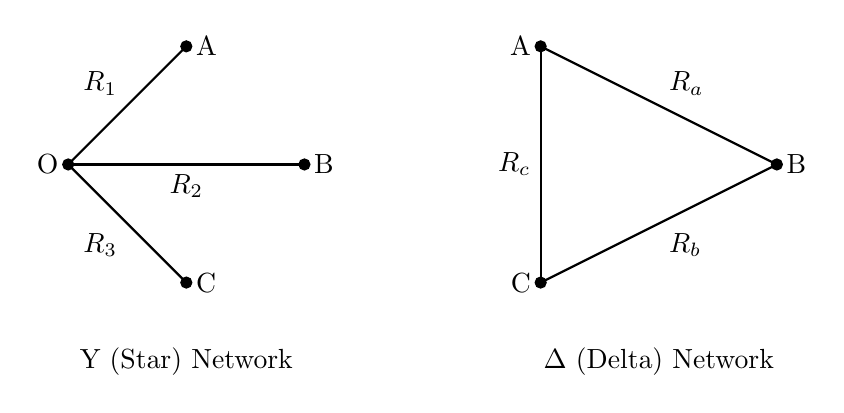
\begin{tikzpicture}
    
    % Y-configuration (Star Network)
    \draw[thick] (0,0) -- (1.5,1.5) node[midway, above left] {$R_1$};
    \draw[thick] (0,0) -- (3,0) node[midway, below] {$R_2$};
    \draw[thick] (0,0) -- (1.5,-1.5) node[midway, below left] {$R_3$};
    \draw[fill=black] (0,0) circle (2pt) node[left] {O};
    \draw[fill=black] (1.5,1.5) circle (2pt) node[right] {A};
    \draw[fill=black] (3,0) circle (2pt) node[right] {B};
    \draw[fill=black] (1.5,-1.5) circle (2pt) node[right] {C};
    \node at (1.5,-2.5) {Y (Star) Network};
    
    % Delta-configuration (Delta Network)
    \draw[thick] (6,1.5) -- (9,0) node[midway, above right] {$R_a$};
    \draw[thick] (9,0) -- (6,-1.5) node[midway, below right] {$R_b$};
    \draw[thick] (6,-1.5) -- (6,1.5) node[midway, left] {$R_c$};
    \draw[fill=black] (6,1.5) circle (2pt) node[left] {A};
    \draw[fill=black] (9,0) circle (2pt) node[right] {B};
    \draw[fill=black] (6,-1.5) circle (2pt) node[left] {C};
    \node at (7.5,-2.5) {\(\Delta \)  (Delta) Network};
    
    \end{tikzpicture}
\end{center}
    
\begin{center}
    \renewcommand{\arraystretch}{1.5} % Adjust row height
    \setlength{\tabcolsep}{12pt} % Adjust column width
    \begin{tabular}{|c|c|}
    \hline
    \textbf{Y to \(\Delta\) Transformation} & \textbf{\(\Delta\) to Y Transformation} \\
    \hline
    $R_a = \frac{R_1 R_2 + R_2 R_3 + R_3 R_1}{R_1}$ & $R_1 = \frac{R_a R_c}{R_a + R_b + R_c}$ \\
    $R_b = \frac{R_1 R_2 + R_2 R_3 + R_3 R_1}{R_2}$ & $R_2 = \frac{R_a R_b}{R_a + R_b + R_c}$ \\
    $R_c = \frac{R_1 R_2 + R_2 R_3 + R_3 R_1}{R_3}$ & $R_3 = \frac{R_b R_c}{R_a + R_b + R_c}$ \\
    \hline
    \end{tabular}
\end{center}



\section{Superconductor}

A superconductor, in most cases can be well modelled by a perfect conductor, that is \(\sigma \rightarrow \infty\). And the most important fact about a superconductor (or a perfect conductor) is that the magnetic flux through the conductor is always constant. This is because if there is a change of magnetic flux, thus an induced emf, the current could get arbitraily large for infinitisimal small emf. In practice, when a magnetic field line try to penetrate through the conductor, a slight emf is induced which is enough to produce an induced current that generate an opposing magnetic field.

If we have a sheet of perfect conductor and put a magnet next to it, currents called ``eddy currents'' appear in the sheet so that no magnetic flux enters. The field lines in this case would look like this:

\onefig{superconductorfieldline}{scale=0.3} 

Since the currents in the magnet and the eddy currents are in opposite directions, they repel and the magnet get levitated above the sheet. If the conductor is not perfect there will be some resistance to the flow of the eddy currents. The currents will tend to die out and the magnet will slowly settle down and the flux of the magnetic field from the magnet would gradually penetrate the conductor.

Eddy currents are best illustrated by the ``pendulum'' set up shown in \cref{eddypen1}.

\twofig{eddypen1}{width=\textwidth}{eddypen2}{width=\textwidth}{eddypen} 

As the metal plate enters the gap of the magnet, there will be eddy current induced in the plate which acts to oppose the change in flux through the plate, so the current s at first bring the plate almost to a dead stop as it starts to enter the field. Then as the currents die down the plate slowly settles to rest at the equilibrium position. The nature of the eddy currents is shown in \cref{eddypen2}.  

If, for instance the copper plate is replace by one which has several narrow slots cut in it, the eddy current effects are drastically reduced, since the currents in each section of the loop have less flux to drive them so the effects of the resistance of each loop are greater. 

\chapter{Operational Amplifiers}

The shematic diagram of an operational amplifier is shown below

\begin{center}
    \begin{circuitikz}
        % Draw the op-amp triangle
        \draw (0,0) node[op amp, noinv input up] (opamp) {};
        
        % Inputs with circles at the ends
        \draw (opamp.-) -- ++(-0.5,0)             node[ocirc, inner sep=1.5pt] {}  node[left] {$V_\text{in}^-$};
        \draw (opamp.+) -- ++(-0.5,0)             node[ocirc, inner sep=1.5pt] {}  node[left] {$V_\text{in}^+$};
        
        % Output with circle at the end
        \draw (opamp.out) -- ++(0.5,0)             node[ocirc, inner sep=1.5pt] {}  node[right] {$V_\text{out}$};
        
        % Power supplies with circles at the ends
        \draw (opamp.up) -- ++(0,0.5)             node[ocirc, inner sep=1.5pt] {}  node[above] {$V_\text{cc}^+$};
        \draw (opamp.down) -- ++(0,-0.5)             node[ocirc, inner sep=1.5pt] {}  node[below] {$V_\text{cc}^-$};
    \end{circuitikz}
\end{center}

In the diagram, \(V_{\text{cc} }^{\pm }  \) are the power supply voltages, which are usually omitted. \(V_{\text{in} }^{\pm }  \) are the input voltages and \(V_{out} \) is the output voltage.   

The characteristic equation of an op-amp is 

\begin{equation}
    V_{\text{out} } = A_{\text{OL}} (V_{\text{in} }^+ - V_{in}^- )  
\end{equation}

Typically, the open-loop voltage gain \(A_{\text{OL}}\) is very large \((\sim 10^{5} )\) , but the output voltage \(V_{\text{out}}\) is limited within a range set by two saturation voltages \(V_{\text{sat}}^{\pm} \approx V_{\text{cc}}^{\pm} \mp 1V\). This implies that any small difference between the op-amp inputs will cause the output to saturate.

\section{Non-Linear Applications}
An op-amp can be used as a comparator: 


\begin{center}
    \begin{circuitikz}
        % Draw the op-amp triangle
        \draw (0,0) node[op amp, noinv input up] (opamp) {};
        
        % Non-inverting input (Vin+)
        \draw (opamp.+) -- ++(-0.5,0) 
            node[ocirc, inner sep=1.5pt] {} 
            node[left] {$V_\text{in}$};
        
        % Inverting input connected to a battery
        \draw (opamp.-) -- ++(-0.5,0) 
            to[battery, l_=1V] ++(0,-1.5)
            node[ground] {};

        % Output (Vout)
        \draw (opamp.out) -- ++(0.5,0) 
            node[ocirc, inner sep=1.5pt] {} 
            node[right] {$V_\text{out}$};
    \end{circuitikz}
\end{center}

If the inverting input signal is fixed at, say \(1V\), then the output voltage will be positive if the input signal is greater than \(1V\), and negative if the input signal is smaller than \(1V\). Since the saturation voltages are reached pratically instantly, we would get a square wave on the output signal in response to some arbitrary input signal wandering around the level of the fixed voltage at the inverting input, as shown in \cref{comparator}. 

\onefig{comparator}{scale=0.3} 

\section{Linear Applications}

We can state the two ``golden rules'' of an ideal linear op-amp:

\begin{enumerate}
    \item The output will do whatever is necessary to make the voltage difference between the inputs zero.\footnote{Note that it does not mean that the op-amp acutally changes the voltage at tis inputs. What it does is ``look'' at its input terminals and swing its output terminal around so that the external feedback betwork brings the input differential to zero.}
    \item No current flows into the inputs.\footnote{But current can flows out of the output.} 
\end{enumerate}

A simple inverting amplifier is shown in \cref{invertingopamp} 

\onefig{invertingopamp}{scale=0.3} 

Since \(B\) is at ground, so by ``golden rule'' 1 \(A\) is also at ground. Therefore the voltage across \(R_2 \) is \(V_{\text{out}} \) and the voltage across \(R_1 \) is \(V_{\text{in}} \). And by rule 2 we have \(\displaystyle \frac{V_{\text{out}} }{R_2 } = - \frac{V_{\text{in}} }{R_1 }  \). 

To understand what is really happening, imagine initially all the terminals are at zero voltage, now \(V_{\text{in}} \) is raised to \(+1V\). Due to the enormous input unbalance, \(V_{\text{out}} \) is dropped to the saturation voltage  

\example{Digital to Analogue Converter.}
{Refer to \cref{dac}, find \(V_{\text{out} } \) in terms of \(V_{\text{in} }\text { and } R \).  }
{Since the inverting input is virtually grounded, so the potential at the position of the switch is always zero regardless of the state of the switch, and can be combined with the true ground at the upper right corner of the diagram.

The swtich simply determine whether the current flowing through each bracnhes flows towards the op-amp, or into the ground. Combining the resistors using simple techniques, the voltages at the top of the resistors at each branches are \(V_{\text{in}, \frac{V_{\text{in} } }{2} }, \frac{V_{\text{in} } }{4}  \text { and } \frac{V_{\text{in} } }{8}  \) respectively. 

Thus the total current flowing towards the op-amp is

\begin{equation}
    I = I_0 + I_1 + I_2 + I_3 = \frac{V_{\text{in} } }{2R}\left( S_0 + \frac{S_1}{2} + \frac{S_2 }{4} + \frac{S_3}{8} \right). 
\end{equation}

The output voltage is thus 

\begin{equation}
    V_{\text{out} } = - IR =  - \frac{V_{\text{in} } }{2}\left( S_0 + \frac{S_1}{2} + \frac{S_2 }{4} + \frac{S_3}{8} \right).
\end{equation}


} 

\onefig{dac}{scale=0.5} 



















































\end{document}